\documentclass[11pt]{article}

\usepackage[a4paper,margin=0.72in]{geometry}
\usepackage[T1]{fontenc}
\usepackage{lmodern}
\usepackage{microtype}
\usepackage{amsmath,amssymb}
\usepackage{booktabs}
\usepackage{tabularx}
\usepackage{xcolor}
\usepackage{titlesec}
\usepackage{enumitem}
\usepackage{hyperref}
\usepackage{tikz}
\usetikzlibrary{positioning}
\usepackage[most]{tcolorbox}

\definecolor{DeepBlue}{HTML}{183A59}
\definecolor{SkyBlue}{HTML}{D9ECF8}
\definecolor{WarmGold}{HTML}{C9932C}
\definecolor{SoftGold}{HTML}{FFF3D8}
\definecolor{Leaf}{HTML}{2E6E5B}
\definecolor{SoftLeaf}{HTML}{DFF1EA}
\definecolor{Ink}{HTML}{17212B}
\definecolor{Muted}{HTML}{5C6670}
\definecolor{LightGray}{HTML}{F4F6F8}
\definecolor{LineGray}{HTML}{D4DAE1}

\hypersetup{
  colorlinks=true,
  linkcolor=DeepBlue,
  urlcolor=Leaf,
  citecolor=WarmGold
}

\setlength{\parindent}{0pt}
\setlength{\parskip}{0.55em}
\setlist[itemize]{leftmargin=1.4em,itemsep=0.2em,topsep=0.2em}
\setlist[enumerate]{leftmargin=1.6em,itemsep=0.2em,topsep=0.2em}

\titleformat{\section}
  {\Large\bfseries\color{DeepBlue}}
  {\thesection}{0.6em}{}
\titleformat{\subsection}
  {\large\bfseries\color{Leaf}}
  {\thesubsection}{0.6em}{}
\titleformat{\subsubsection}
  {\normalsize\bfseries\color{WarmGold}}
  {\thesubsubsection}{0.5em}{}

\newtcolorbox{physbox}[2][]{
  enhanced,
  colback=SkyBlue,
  colframe=DeepBlue,
  coltitle=white,
  title=\textbf{#2},
  fonttitle=\bfseries,
  arc=2mm,
  boxrule=0.8pt,
  left=7pt,right=7pt,top=7pt,bottom=7pt,
  #1
}

\newtcolorbox{guidebox}[2][]{
  enhanced,
  colback=SoftLeaf,
  colframe=Leaf,
  coltitle=white,
  title=\textbf{#2},
  fonttitle=\bfseries,
  arc=2mm,
  boxrule=0.8pt,
  left=7pt,right=7pt,top=7pt,bottom=7pt,
  #1
}

\newtcolorbox{warnbox}[2][]{
  enhanced,
  colback=SoftGold,
  colframe=WarmGold,
  coltitle=white,
  title=\textbf{#2},
  fonttitle=\bfseries,
  arc=2mm,
  boxrule=0.8pt,
  left=7pt,right=7pt,top=7pt,bottom=7pt,
  #1
}

\newcommand{\code}[1]{\texttt{#1}}
\newcommand{\E}{\mathcal{E}}
\newcommand{\dd}{\mathrm{d}}

\begin{document}

\begin{titlepage}
\centering
\vspace*{1.0cm}
{\Huge\bfseries\color{DeepBlue} GCascadeV5}\\[0.25cm]
{\LARGE\bfseries Physics-Oriented Code Manual}\\[0.45cm]
{\large Gamma rays, electrons, and the structure of the Python implementation}\\[1.0cm]

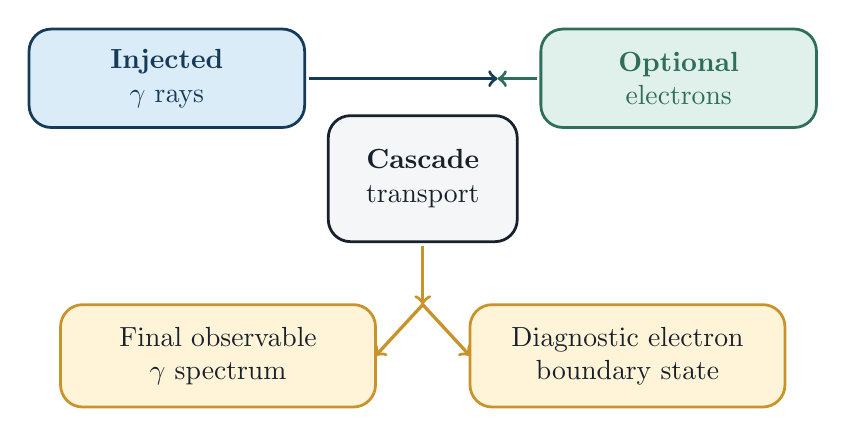
\begin{tikzpicture}[x=1cm,y=1cm]
  \draw[rounded corners=8pt,fill=SkyBlue,draw=DeepBlue,line width=1pt] (-5,0) rectangle (-1.5,1.25);
  \node[align=center,text=DeepBlue] at (-3.25,0.62) {\bfseries Injected\\ $\gamma$ rays};
  \draw[rounded corners=8pt,fill=SoftLeaf,draw=Leaf,line width=1pt] (1.5,0) rectangle (5,1.25);
  \node[align=center,text=Leaf] at (3.25,0.62) {\bfseries Optional\\ electrons};
  \draw[->,line width=1.2pt,color=DeepBlue] (-1.45,0.62) -- (0.95,0.62);
  \draw[->,line width=1.2pt,color=Leaf] (1.45,0.62) -- (0.95,0.62);
  \draw[rounded corners=8pt,fill=LightGray,draw=Ink,line width=1pt] (-1.2,-1.45) rectangle (1.2,0.15);
  \node[align=center,text=Ink] at (0,-0.65) {\bfseries Cascade\\ transport};
  \draw[->,line width=1.2pt,color=WarmGold] (0,-1.5) -- (0,-2.25);
  \draw[rounded corners=8pt,fill=SoftGold,draw=WarmGold,line width=1pt] (-4.6,-3.55) rectangle (-0.6,-2.25);
  \node[align=center,text=Ink] at (-2.6,-2.9) {Final observable\\ $\gamma$ spectrum};
  \draw[rounded corners=8pt,fill=SoftGold,draw=WarmGold,line width=1pt] (0.6,-3.55) rectangle (4.6,-2.25);
  \node[align=center,text=Ink] at (2.6,-2.9) {Diagnostic electron\\ boundary state};
  \draw[->,line width=1.2pt,color=WarmGold] (0,-2.25) -- (-0.6,-2.9);
  \draw[->,line width=1.2pt,color=WarmGold] (0,-2.25) -- (0.6,-2.9);
\end{tikzpicture}

\vfill
{\large Generated for the repository}\\[0.1cm]
{\code{/Users/antonio/Desktop/Research/GCascadeV5}}\\[0.55cm]
{\large April 17, 2026}
\end{titlepage}

\tableofcontents
\newpage

\section{How to Read This Manual}

This guide is written for physicists first. It explains what each file in the
code does, but it starts from the physical picture: particles injected at some
redshift, interactions with background light, and spectra transported down to
redshift zero.

Where a programming word would normally appear, this manual uses a more
physical phrase. For example, instead of saying ``API'', it says
\emph{user-facing functions}. Instead of saying ``cache'', it says
\emph{recently remembered table slices}. The goal is that the code feels like a
set of instruments for evolving spectra, not a maze of software machinery.

\begin{guidebox}{Most useful files for physicists}
\begin{itemize}
  \item \code{api.py}: the functions you call from a notebook.
  \item \code{physics.py}: physical constants, cosmology, and the shared grids.
  \item \code{transport.py}: the new gamma/electron cascade evolution.
  \item \code{state.py}: the active library tables and current EBL/magnetic-field settings.
  \item \code{bundle.py}: the runtime library layout and manifest handling.
\end{itemize}
\end{guidebox}

\section{The Physical Problem}

GCascadeV5 evolves spectra on a fixed logarithmic energy grid,
\[
  E_i \in [10^{-1},10^{12}]~{\rm GeV}, \qquad i=0,\ldots,299 .
\]
The redshift path is divided into many small steps. At each step the code
updates two spectra:
\[
  \Phi_\gamma(E_i,z), \qquad \Phi_e(E_i,z).
\]

The previous on-the-spot approximation kept only $\Phi_\gamma$. Whenever a
gamma ray pair-produced an electron/positron pair, the electron energy was
assumed to return instantly to photons by inverse Compton scattering at the
same redshift step. V5 now keeps the electron spectrum alive:
\[
  \gamma \longrightarrow e^\pm,
  \qquad
  e^\pm \longrightarrow e^\pm+\gamma,
\]
so delayed cooling, repeated scattering, and magnetic-field losses can be
represented more faithfully.

\begin{physbox}{One redshift step, in words}
\begin{enumerate}
  \item Gamma rays survive or pair-produce on the CMB/EBL.
  \item Absorbed gamma-ray power is deposited into electrons.
  \item Electrons inverse-Compton scatter, producing photons and lower-energy electrons.
  \item A magnetic field may remove some electron energy as synchrotron loss.
  \item Both spectra are redshifted to the next lower redshift window.
\end{enumerate}
\end{physbox}

\subsection{The Main Equations}

A convenient way to read the code is to view one short propagation interval as
a set of linear spectral maps.

Photon survival through pair production is treated as
\[
  \Phi_\gamma^{\rm surv}(E)
  =
  \exp[-\Delta s/\lambda_{\gamma\gamma}(E,z)]\,
  \Phi_\gamma(E),
\]
where $\lambda_{\gamma\gamma}$ is the pair-production mean free path and
$\Delta s$ is the propagation length represented by the fine step.

The absorbed photon spectrum is
\[
  \Delta\Phi_\gamma(E)
  =
  \Phi_\gamma(E)-\Phi_\gamma^{\rm surv}(E).
\]
It is redistributed into electrons by the pair-production kernel
$K_{\gamma\rightarrow e}$:
\[
  \Phi_e \leftarrow
  \Phi_e + K_{\gamma\rightarrow e}\,\Delta\Phi_\gamma .
\]

Electrons inverse-Compton scatter with a similar survival factor,
\[
  \Phi_e^{\rm surv}(E)
  =
  \exp[-\Delta s/\lambda_{\rm IC}(E,z)]\,
  \Phi_e(E).
\]
The scattered part,
\[
  \Delta\Phi_e=\Phi_e-\Phi_e^{\rm surv},
\]
feeds both photons and outgoing electrons:
\[
  \Phi_\gamma \leftarrow \Phi_\gamma + K_{e\rightarrow\gamma}\,\Delta\Phi_e,
\]
\[
  \Phi_e \leftarrow \Phi_e^{\rm surv}
  + K_{e\rightarrow e}\,\Delta\Phi_e .
\]

When a magnetic field is active, synchrotron losses compete with ICS. The code
uses the same physical scaling as the previous V5 implementation:
\[
  \left.\frac{\dd E}{\dd t}\right|_{\rm syn}
  =
  \frac{1}{e}
  \frac{4}{3}\sigma_T c
  \frac{B(z)^2}{2\mu_0}
  \gamma_e^2,
  \qquad
  B(z)=B_0(1+z)^\alpha .
\]
The removed energy is not injected into the gamma-ray spectrum; it is recorded
as diagnostic synchrotron energy loss.

\section{What Users Call}

The most important user-facing functions are:

\begin{center}
\begin{tabularx}{0.95\linewidth}{@{}lX@{}}
\toprule
\textbf{Function} & \textbf{Physical meaning} \\
\midrule
\code{RedshiftPoint} & Only cosmological redshifting of a point-source spectrum. \\
\code{AttenuatePoint} & Redshifting plus pair-production absorption. \\
\code{CascadePoint} & Full gamma/electron cascade transport for one source. \\
\code{RedshiftDiffuse} & Redshift-only diffuse population. \\
\code{AttenuateDiffuse} & Absorbed diffuse population. \\
\code{CascadeDiffuse} & Full cascade for non-evolving diffuse population. \\
\code{CascadeEvolving} & Full cascade for redshift-dependent injection. \\
\bottomrule
\end{tabularx}
\end{center}

By default, the cascade functions return only the final gamma-ray spectrum,
so old notebooks keep working:
\[
  \phi_\gamma(E) = \code{CascadePoint(gamma\_inj, z)} .
\]
If the full state is desired:
\[
  \code{return\_state=True}
\]
returns a \code{CascadeResult} with final photons, final electrons, and
diagnostics.

\begin{warnbox}{How to think about the electron output}
\code{result.electron} is a diagnostic extragalactic boundary-state spectrum.
It is not a direct charged-particle flux at Earth. Galactic magnetic fields,
angular spreading, time delays, and local transport are outside this code.
\end{warnbox}

\section{The Library Tables}

The code reads precomputed physics tables from \code{LibrariesV5}. The current
library format is HDF5, with one manifest:
\[
  \code{LibrariesV5/bundle\_manifest.json}.
\]

The schema-v2 runtime files include:
\begin{itemize}
  \item pair-production attenuation tables,
  \item pair-production spectra,
  \item ICS interaction rates,
  \item ICS photon spectra,
  \item outgoing-electron ICS spectra,
  \item ICS energy-loss rates for checks and low-energy fallback.
\end{itemize}

All ICS-related tables are now part of \code{LibrariesV5} itself. Ordinary
cascade runs read one library only: the main HDF5 bundle.

\section{A Visual Map of the Code}

\begin{center}
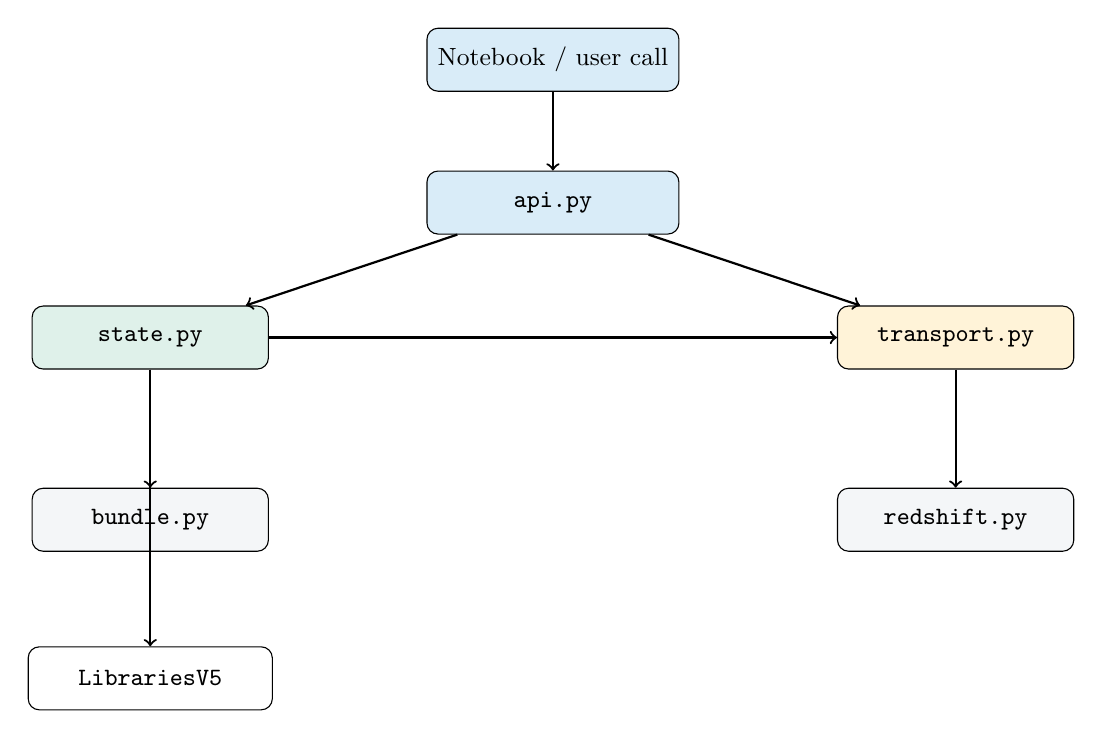
\begin{tikzpicture}[node distance=1.0cm, every node/.style={font=\small}]
  \node[draw,rounded corners,fill=SkyBlue,minimum width=3.2cm,minimum height=0.8cm] (user) {Notebook / user call};
  \node[draw,rounded corners,fill=SkyBlue,below=of user,minimum width=3.2cm,minimum height=0.8cm] (api) {\code{api.py}};
  \node[draw,rounded corners,fill=SoftLeaf,below left=0.9cm and 2.0cm of api,minimum width=3.0cm,minimum height=0.8cm] (state) {\code{state.py}};
  \node[draw,rounded corners,fill=SoftGold,below right=0.9cm and 2.0cm of api,minimum width=3.0cm,minimum height=0.8cm] (transport) {\code{transport.py}};
  \node[draw,rounded corners,fill=LightGray,below=1.5cm of state,minimum width=3.0cm,minimum height=0.8cm] (bundle) {\code{bundle.py}};
  \node[draw,rounded corners,fill=LightGray,below=1.5cm of transport,minimum width=3.0cm,minimum height=0.8cm] (redshift) {\code{redshift.py}};
  \node[draw,rounded corners,fill=white,below=1.2cm of bundle,minimum width=3.1cm,minimum height=0.8cm] (h5) {\code{LibrariesV5}};
  \draw[->,thick] (user) -- (api);
  \draw[->,thick] (api) -- (state);
  \draw[->,thick] (api) -- (transport);
  \draw[->,thick] (state) -- (bundle);
  \draw[->,thick] (state) -- (h5);
  \draw[->,thick] (transport) -- (redshift);
  \draw[->,thick] (state) -- (transport);
\end{tikzpicture}
\end{center}

\newpage
\section{Every File in \code{src/gcascade\_v5}}

\subsection{\code{\_\_init\_\_.py}: the package doorway}

This is the doorway into the package. When a notebook says
\[
  \code{import gcascade\_v5 as gc},
\]
this file decides what appears under the name \code{gc}. It exposes the main
functions and live status values such as the currently selected EBL model.

\textbf{Physical role:} none directly. It is the front door to the instruments.

\textbf{Important detail:} \code{gc.EBLindex} is not a fixed number copied at
import time. It always reflects the currently active EBL model.

\subsection{\code{core.py}: the simple re-export shelf}

This file is intentionally tiny. It gathers the main user-facing functions from
\code{api.py}.

\textbf{Physical role:} none directly. It keeps the import surface tidy.

\subsection{\code{api.py}: the laboratory control panel}

This is where physicists interact with the code. It checks that spectra have
the right shape, chooses the requested calculation, asks \code{state.py} for
the right physics tables, and applies the final point-source or diffuse
normalization.

For point sources, the final photon spectrum is scaled by the luminosity
distance:
\[
  \phi_\gamma(E_0)
  =
  \frac{(1+z_s)^2}{4\pi d_L^2}
  \Phi_\gamma(E_0,z=0).
\]
Diffuse calculations use the usual $1/(4\pi)$ angular factor after integrating
the source distribution.

\textbf{Main functions:}
\begin{itemize}
  \item \code{RedshiftPoint}, \code{RedshiftDiffuse}, \code{RedshiftEvolving}
  \item \code{AttenuatePoint}, \code{AttenuateDiffuse}, \code{AttenuateEvolving}
  \item \code{CascadePoint}, \code{CascadeDiffuse}, \code{CascadeEvolving}
  \item \code{changeEBLModel}, \code{changeMagneticField}
  \item \code{get\_bundle\_info}, \code{reset\_factory\_settings}
\end{itemize}

\textbf{How to read it:} search for the function you call from a notebook. The
body of that function shows the calculation sequence in plain order: validate
input, load tables, propagate, normalize, return.

\subsection{\code{state.py}: the active observing setup}

This file remembers which EBL model is active, which HDF5 library is being
used, which redshift tables are loaded, and what magnetic-field parameters are
currently selected.

An analogy: if \code{api.py} is the control panel, \code{state.py} is the
current experimental setup. It knows which target, filters, and calibration
tables are installed.

\textbf{Important physical quantities held here:}
\begin{itemize}
  \item pair-production attenuation factors,
  \item ICS attenuation factors,
  \item redshift interpolation tables,
  \item pair-production spectra,
  \item ICS photon and electron spectra,
  \item $B_0$ and $\alpha$ in $B(z)=B_0(1+z)^\alpha$.
\end{itemize}

Because the HDF5 kernels are large, \code{state.py} only keeps a few recently
used redshift slices ready at a time. This is a practical memory-saving detail,
not a change in the physics.

\subsection{\code{transport.py}: the gamma/electron cascade engine}

This is the physical heart of the new V5 cascade. It advances
\[
  \begin{pmatrix}\Phi_\gamma\\ \Phi_e\end{pmatrix}
\]
from high redshift to low redshift.

\textbf{Central operation:}
\[
  \Phi_\gamma \rightarrow
  \Phi_\gamma^{\rm surv}
  + K_{e\rightarrow\gamma}\Delta\Phi_e,
\]
\[
  \Phi_e \rightarrow
  \Phi_e^{\rm surv}
  + K_{\gamma\rightarrow e}\Delta\Phi_\gamma
  + K_{e\rightarrow e}\Delta\Phi_e .
\]

\textbf{Main functions:}
\begin{itemize}
  \item \code{transport\_step}: one fixed-redshift transport step.
  \item \code{propagate\_point\_transport}: point-source cascade.
  \item \code{propagate\_diffuse\_transport}: diffuse cascade.
  \item \code{propagate\_evolving\_transport}: redshift-evolving source cascade.
  \item \code{synchrotron\_loss\_rates}: computes synchrotron loss for $B(z)$.
  \item \code{spectrum\_energy}: integrates a spectrum over the energy grid.
\end{itemize}

\textbf{Low-energy behavior:} when discrete ICS scattering becomes too small
relative to the logarithmic energy bin width, the code uses a conservative
continuous-loss style fallback so electrons do not get numerically stuck in a
single bin.

\subsection{\code{results.py}: the cascade notebook}

This file defines \code{CascadeResult}, the object returned when
\code{return\_state=True}. It contains:
\begin{itemize}
  \item \code{gamma}: the final gamma-ray spectrum,
  \item \code{electron}: the diagnostic electron spectrum,
  \item \code{diagnostics}: energy bookkeeping,
  \item \code{metadata}: run labels and normalization information.
\end{itemize}

\textbf{Physical role:} it keeps all final spectra and bookkeeping in one place
so the gamma observable and electron diagnostic do not get confused.

One diagnostic deserves special mention: \code{redshift\_energy\_lost}. This is
not a numerical error. It is the energy removed by cosmological expansion while
the particles slide from one redshift window to the next.

\subsection{\code{physics\_tables.py}: transport-table source checks}

This file checks that a \code{LibrariesV5} bundle contains the transport tables
needed by the gamma$+$electron cascade and loads them when the bundle is used as
a source during library rebuilding.

\textbf{Physical tables checked here:}
\begin{itemize}
  \item \code{ics\_imfp}: ICS interaction rates,
  \item \code{ics\_gamma\_packed}: ICS photon spectra,
  \item \code{ics\_electron\_packed}: outgoing-electron spectra,
  \item \code{pp\_packed}: pair-production spectra,
  \item \code{dEdt\_ics}: ICS loss-rate tables.
\end{itemize}

\subsection{\code{physics.py}: shared constants, cosmology, and grids}

This file collects the physical constants and common grids used throughout the
code:
\begin{itemize}
  \item the electron rest mass,
  \item the Thomson cross section,
  \item the present CMB temperature,
  \item the logarithmic energy grid,
  \item the pretabulated redshift windows,
  \item the Hubble expansion law and luminosity distance.
\end{itemize}

\textbf{Why it matters physically:} it gives one single place where the basic
background assumptions of the calculation are defined.

\subsection{\code{bundle.py}: the library archivist}

This file describes the HDF5 library format and reads the manifest that tells
the code where each runtime table lives.

\textbf{Physical content written into runtime files:}
\begin{itemize}
  \item $\lambda_{\gamma\gamma}^{-1}$ and gamma survival factors,
  \item $K_{\gamma\rightarrow e}$ pair-production spectra,
  \item $\lambda_{\rm IC}^{-1}$ and electron survival factors,
  \item $K_{e\rightarrow\gamma}$ ICS photon spectra,
  \item $K_{e\rightarrow e}$ outgoing-electron spectra,
  \item $\dd E/\dd t$ ICS loss-rate tables.
\end{itemize}

The file also records provenance in \code{bundle\_manifest.json}, so one can
see where the runtime tables came from.

\subsection{\code{redshift.py}: cosmological energy shifting}

This file applies the mapping between neighboring redshift windows. In physical
terms,
\[
  E_{\rm emitted}=E_{\rm observed}\frac{1+z_{\rm high}}{1+z_{\rm low}} .
\]
The spectrum is interpolated in logarithmic space, which is appropriate for the
wide logarithmic energy grid.

\textbf{Used by:} redshift-only calculations, attenuation calculations, and the
new gamma/electron transport.

\subsection{\code{attenuation.py}: absorption without regeneration}

This file evolves photons with pair-production absorption but without secondary
cascade regeneration. The basic operation is:
\[
  \Phi_\gamma(E) \leftarrow
  \exp[-\tau_{\gamma\gamma}(E)]\Phi_\gamma(E).
\]

It is useful when one wants to separate:
\[
  \text{redshift only}
  \quad \rightarrow \quad
  \text{redshift + absorption}
  \quad \rightarrow \quad
  \text{full cascade}.
\]

\subsection{\code{config.py}: progress messages}

This file controls:
\begin{itemize}
  \item whether progress messages are shown,
  \item simple progress bars.
\end{itemize}

\textbf{Physical role:} none. It affects convenience and speed only.

\subsection{\code{tutorial\_support.py}: small notebook helpers}

This file contains small functions used by tutorials to check whether a bundle
exists and where its manifest should be. It has no cascade physics.

\section{Generated Files in the Code Directory}

\subsection{\code{.DS\_Store}}

A macOS Finder metadata file. It has no physical or numerical meaning.

\subsection{\code{\_\_pycache\_\_/}}

Python creates these files automatically after imports. They can be deleted
safely; the computer will regenerate them when needed.

\section{Repository Folders Outside the Code Directory}

\begin{center}
\begin{tabularx}{0.96\linewidth}{@{}lX@{}}
\toprule
\textbf{Folder} & \textbf{Meaning} \\
\midrule
\code{LibrariesV5} & Main HDF5 physics library used by normal runs. \\
\code{tests} & Checks for physics-table loading, transport behavior, and energy conservation. \\
\code{benchmarks} & Runtime timing helpers. \\
\code{tutorial.ipynb} & Interactive tutorial for users. \\
\code{safe\_snapshots} & Preserved baseline copy of the previous V5 Python code. \\
\bottomrule
\end{tabularx}
\end{center}

\section{The Flow of \code{CascadePoint}}

\begin{enumerate}
  \item The user supplies a gamma spectrum, optional electron spectrum, and source redshift.
  \item \code{api.py} checks shapes and redshift range.
  \item \code{state.py} opens the active EBL tables in \code{LibrariesV5}.
  \item \code{transport.py} evolves $\Phi_\gamma$ and $\Phi_e$ down the redshift grid.
  \item \code{redshift.py} remaps both spectra between redshift windows.
  \item \code{api.py} applies the luminosity-distance factor.
  \item The user receives either $\phi_\gamma$ or the full \code{CascadeResult}.
\end{enumerate}

\section{Testing Commands}

Default checks:
\[
  \code{GCASCADE\_PROGRESS=0\ PYTHONPATH=src\ python3\ -m\ pytest\ -q}.
\]

Focused electron-transport checks:
\[
  \code{PYTHONPATH=src\ python3\ -m\ pytest\ -q\ tests/test\_transport.py}.
\]

\section{Practical Advice for Future Physics Work}

\begin{guidebox}{Where to modify the code}
\begin{itemize}
  \item Change cascade physics in \code{transport.py}.
  \item Add new HDF5 table types through \code{bundle.py} and \code{state.py}.
  \item Add new transport-table validation rules in \code{physics\_tables.py}.
  \item Add user-facing controls in \code{api.py}.
  \item Keep the energy bookkeeping tests updated whenever transport physics changes.
\end{itemize}
\end{guidebox}

\begin{warnbox}{Most important conceptual distinction}
\[
  \text{Old V5: photons only, electrons cool immediately.}
\]
\[
  \text{New V5: photons and electrons are both evolved.}
\]
This is the central structural change. Most code changes follow from this one
physics decision.
\end{warnbox}

\end{document}
